
\subsection*{\textbf{Question 5.d}}
\begin{quote}

\textbf{Problem}
\begin{quote}
Write your own FFT algorithm; check that your code works with a 1D function (no Gaussian) by making a plot of the FFt and compare your result with a python package and the analytical FFT of your function. In the rest of this exercise you need to use your own FFT. 
\end{quote}

\textbf{Solution} 
\begin{quote}
The created implementation of the FFT consist of an recursive implementation with the Cooley-Tukey algorithm. The implementation doesn't store the data inplace, but in a new array. This choice was made to prevent he input array from being modified. One consequence of this choice is that the input array does not have to be reverse bit shifted. 
\\
The implementation is compared with the numpy implementation. The function that is chosen to fourier transform is the cosine\footnote{The given expression contains a proportional sign as the pre-factor depends on the definition of the Fourier transformation.},

\begin{equation}
\mathcal{F}(\cos(2 \pi At) ]\propto 0.5(\delta(f - A) + \delta(f + A))
\end{equation}
\\
The code for the FFT can be found on page .. in the file .... The code that compares the self written implementation with the numpy implementation and the analytical solution can be found below.  
\newpage

%
%\newpage
%\end{quote}

\textbf{Code - slices}
\begin{quote}
The code that creates the plots for the comparison of the self written FFT with the numpy implementation and the analytical solution.
%The code that creates the slices, cell 0 and cell 4 in a 3D grid of size 16.
\lstinputlisting[firstline = 108, lastline=137]{./Code/assigment_5.py}
\end{quote}

\newpage
\textbf{Plot - Comparison}
\begin{quote}

\begin{figure}[!ht]
\centering
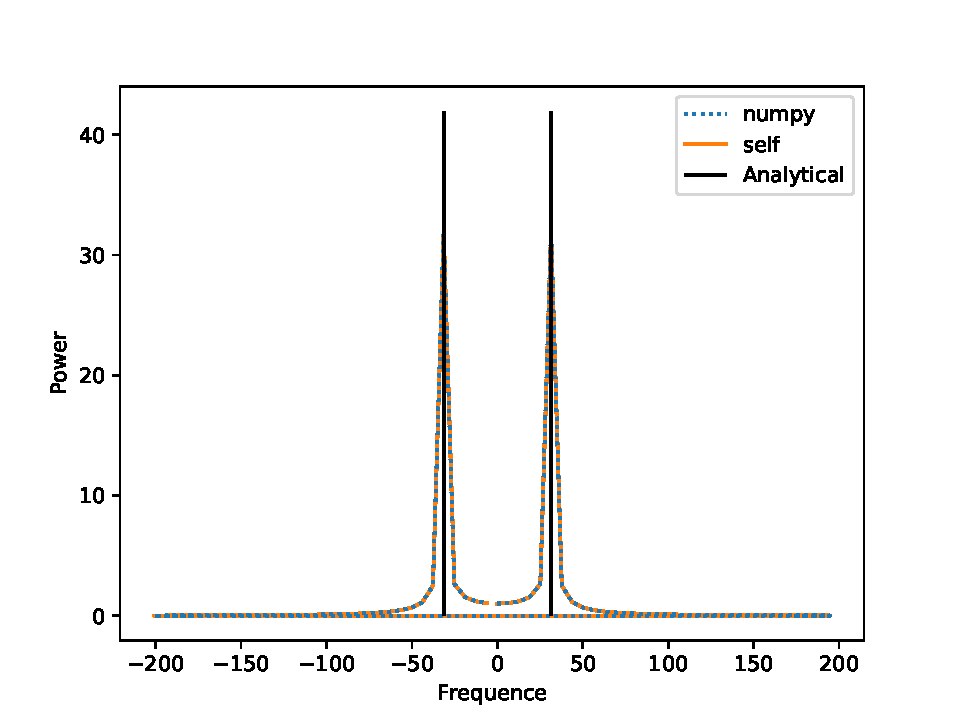
\includegraphics[width=14cm, height=8.5cm]{./Plots/5d_fourier.pdf}
\caption{The own implementation of the FFT (orange), the numpy implementation (blue) and the analytical fft (black). The plot shows that there is now visible deviation from the numpy version. It can also be seen that both the numpy and the self written implementation do not correctly represent the peak of the delta function. This is expected as it would require an infinite amount of samples to obtain the exact same result. }
\end{figure}
\end{quote}
%\newpage


\end{quote}
\end{quote}











